\documentclass[conference]{IEEEtran}

\usepackage{amsmath,amssymb}
\usepackage{enumitem}
\usepackage{stmaryrd}
\usepackage{amsthm}
\usepackage{booktabs}
\usepackage{xcolor}
\usepackage{tikz}
\usetikzlibrary{arrows.meta,positioning}
\usepackage{quantikz}
\usepackage{algorithm}
\usepackage{algpseudocode}
\usepackage[hidelinks]{hyperref}

\newcommand{\code}[1]{\texttt{#1}}
\newcommand{\file}[1]{\texttt{#1}}
\newcommand{\Algo}[1]{\textup{\textsc{#1}}}

\theoremstyle{plain}
\newtheorem{theorem}{Theorem}
\newtheorem{lemma}{Lemma}
\newtheorem{proposition}{Proposition}
\newtheorem{definition}{Definition}
\newtheorem{corollary}{Corollary}

\begin{document}

\title{From Truth Table to Quantum Circuit: K-Map-Guided Toffoli Synthesis\\with Disjoint Cube Covers}
\author{\IEEEauthorblockN{Arham Akhtar}
\IEEEauthorblockA{Lightrider}}

\maketitle

\begin{abstract}
Textbook Karnaugh-map grouping is unsound when applied unchanged to
reversible circuits: it permits overlapping groups because a classical
AND-OR circuit \emph{sets} its output, but a Toffoli-based circuit
\emph{flips} its output one gate at a time, so overlapping groups cancel
each other on their shared cells. We give a greedy algorithm that instead
produces an \emph{exact disjoint} cube cover of each output's on-set,
prove it correct, and use it to synthesize a Toffoli-based circuit
directly from a truth table, with correctness both proved and checked by
exhaustive simulation.
We further give two independent optimizations -- sharing a term between
outputs via a scratch ancilla, and deriving one output from another via a
cheap XOR correction -- each with its own correctness proof, plus a
peephole pass that cancels the adjacent $X$ gates left behind by
complemented controls. All claims are validated both by proof and by
thousands of randomized simulation trials, and every benchmark circuit is
checked by exhaustive classical replay. A worked one-bit full adder is
carried through every stage of the pipeline; a two-bit ripple-carry adder
shows derivation nearly halving gate count by rediscovering the standard
identity that a ripple adder's sum bit is its inputs XORed with the
incoming carry; and $X$-cancellation removes up to $47\%$ of the gates on
wide single-output predicates where the other optimizations do nothing.
Choosing derivations by their gate count after cancellation, and
reordering terms with a simple local search, take the full adder from
$23$ to $14$ gates and the ripple adder from $126$ to $31$.
We connect circuit size to quantum-hardware cost through the standard
Toffoli decomposition and quantum-cost metric, compare against published
RevLib results on \texttt{3\_17} and \texttt{rd32}, and run tweedledum's
ESOP-based and transformation-based synthesizers on the same eleven
functions. That comparison is unfavorable and we report it as such: our
out-of-place construction is $2.2\times$ and $3.5\times$ larger in gate
count than the published in-place MCT circuits for \texttt{3\_17} and
\texttt{rd32}, and tweedledum's out-of-place ESOP circuits have fewer gates
on eight of the eleven functions. This is the price of an end-to-end
correctness proof short enough to check by hand.
\end{abstract}

\begin{IEEEkeywords}
reversible logic synthesis, Karnaugh maps, Toffoli gates, Boolean
hypercube, disjoint cube cover, quantum circuit synthesis, quantum cost
\end{IEEEkeywords}

% =====================================================================
\section{Introduction}
% =====================================================================

Two families of quantum algorithms need correct reversible circuits
synthesized from ordinary truth tables: Grover-style search, whose oracle
must flip a target qubit iff a classical predicate $f(x)=1$, and
Shor-style arithmetic, whose modular adders are chains of one-bit full
adders. Hand-deriving such a circuit is tedious and, as we show in
Section~\ref{sec:disjoint}, easy to get silently wrong: the natural
technique, Karnaugh-map grouping, is taught for circuits that \emph{set}
their output and does not carry over safely to circuits that \emph{flip}
it.

Every gate this paper emits has a fixed, textbook decomposition into the
native gates of a superconducting or trapped-ion device, or into
Clifford+T, with a well-defined \emph{quantum cost}
(Section~\ref{sec:devices}), so gate count is tied to the two-qubit gate
count, depth, and T-count a device must execute.
Section~\ref{sec:benchmarks} compares against published RevLib circuits
and against an established synthesis library run on the same functions.

This paper makes six contributions. (1) A greedy algorithm producing an
exact \emph{disjoint} cube cover of a Boolean function's on-set, proved
correct (Theorem~\ref{thm:exactness}) and validated over $2000$ randomized
on-sets. (2) A direct, proven-correct construction (Theorem
\ref{thm:correctness}) mapping such a cover to a Toffoli-based circuit.
(3) An ancilla-sharing optimization for terms common to two or more
outputs (Lemma~\ref{lem:sharing}), and an independent output-derivation
optimization that builds one output from another via a cheap XOR
correction (Lemma~\ref{lem:derive}), both proved correct and validated.
(4) A peephole pass that cancels adjacent $X$ gates, proved
function-preserving (Lemma~\ref{lem:xcancel}) and validated, which is the
only one of these optimizations that helps on wide single-output
predicates; derivation and sharing chosen by gate count after this pass;
and a term-ordering local search (Lemma~\ref{lem:reorder}) that leaves
the pass more to cancel. (5) A
worked one-bit full adder carried through every stage, and a two-bit
ripple-carry adder demonstrating a substantial reduction from derivation
and cancellation together. (6) An evaluation across eleven functions of
two to eight inputs, including a head-to-head against published MCT
circuits for \texttt{3\_17} and \texttt{rd32} and against tweedledum run on
all eleven, that reports gate count and quantum cost and states plainly
where our construction is larger. A
reference Python implementation, including scripts that regenerate every
number in this paper, is available at
\url{https://github.com/ArhamAkhtarAlam/toffoli-synthesis-final-paper}.

% =====================================================================
\section{Related Work}
\label{sec:related}
% =====================================================================

\subsection{Classical minimization and the reversibility obstruction}
Karnaugh's map~\cite{karnaugh1953} and the algebraic Quine--McCluskey
procedure~\cite{quine1952,mccluskey1956} find a minimal sum-of-products
cover of a Boolean function and explicitly permit overlapping groups,
since a classical AND-OR network sets its output. The Toffoli
gate~\cite{toffoli1980} and the elementary reversible/quantum gate set are
due to Barenco et al.~\cite{barenco1995} and covered in Nielsen and
Chuang~\cite{nielsen2000}. Every gate we use is drawn from exactly that
elementary set, so the decomposition and cost arguments of
Section~\ref{sec:devices} apply without modification.

\subsection{Reversible-logic synthesis techniques}
Reversible-logic synthesis from truth tables falls broadly into four
families~\cite{saeedi2013}. \emph{Transformation-based} synthesis, pioneered by Miller,
Maslov, and Dueck~\cite{miller2003}, repeatedly applies the gate that
moves the current state closest to the target permutation, in either
direction, and is the de facto baseline the field still benchmarks
against. \emph{ESOP-based} synthesis (e.g.\ EXORCISM-4~\cite{mishchenko2001})
targets Exclusive-or Sum-Of-Products forms, which are automatically safe
for XOR-accumulating gates; our disjoint cube cover is a restricted case
of ESOP (no overlap at all), traded for a short, elementary correctness
proof -- general ESOP minimizers search a strictly larger space and can
find smaller circuits at the cost of a harder correctness argument.
\emph{BDD-based} synthesis~\cite{wille2009bdd} emits
gates per node of a decision diagram. \emph{Exact/SAT-based} synthesis
asks a solver for a $k$-gate circuit, guaranteeing gate-optimality but
scaling only to small functions; Gro{\ss}e et al.'s exact synthesis of
elementary quantum gate circuits~\cite{grosse2008} is an instance, and we
compare against its published \texttt{3\_17} result in
Section~\ref{sec:benchmarks}. Our method is none of these: a direct
construction whose only search is greedy (cube growth, derivation choice,
term order), chosen so that
Theorems~\ref{thm:exactness}--\ref{thm:correctness} have short, checkable
proofs. Downstream of such synthesis, quantum compilers such as
t$|$ket$\rangle$~\cite{sivarajah2020} and Qiskit's
transpiler~\cite{qiskit2024} map circuits to a device's gate set and
connectivity, and exact search finds depth-optimal Clifford+T circuits for
small operations such as the Toffoli gate~\cite{amy2013}; our circuits
are an input to that stage, not a replacement for it.

\subsection{Benchmarks and tooling}
RevLib~\cite{revlib2008} is the standard public repository of reversible-
function benchmarks and published circuit realizations, and is the
source of the \texttt{3\_17} and \texttt{rd32} functions and the published
circuits we compare against in Section~\ref{sec:benchmarks}. On the tooling side,
Qiskit~\cite{qiskit2024} exposes truth-table-to-circuit synthesis through
\code{PhaseOracle} and the legacy \code{TruthTableOracle}; RevKit~\cite{soeken2012revkit}
implements ESOP-based synthesis (\code{esopbs}) and several of the
families above; tweedledum~\cite{schmitt2022} provides a reusable synthesis and optimization
library consumed by several front ends; and SyReC~\cite{wille2016syrec} compiles a small
hardware-description language directly to reversible circuits. We run
tweedledum's PKRM, PPRM, and transformation-based synthesizers on our
benchmarks in Section~\ref{sec:tools}. These
tools target production use and gate-count optimality; our contribution
is complementary -- a minimal construction simple enough to prove by
hand and check end to end by exhaustive simulation, intended as a well-specified building block
rather than a replacement for them.

% =====================================================================
\section{Preliminaries}
% =====================================================================

\begin{definition}[Truth table]
For $n$ inputs and $m$ outputs, a truth table is $f:\{0,1\}^n\to\{0,1\}^m$,
listed MSB-first: row $i$ is the binary expansion of $i$.
\end{definition}

\begin{definition}[Pattern and cube]
A pattern $p\in\{0,1,-\}^n$ denotes the sub-cube
$\llbracket p \rrbracket = \{x\in\{0,1\}^n : x_k=p_k \text{ whenever } p_k \ne {-}\}$.
$|\llbracket p \rrbracket| = 2^d$ for $d$ dashes in $p$.
\end{definition}

\begin{definition}[Gate set]
\label{def:gates}
Let $w=n+m+a$ ($n$ inputs, $m$ outputs, $a$ ancillas, outputs/ancillas
initialized to $\ket 0$). Circuits act on $\{0,1\}^w$ via: $X_S$ (flip every
wire in $S$) and $C^kX_{c_1,\dots,c_k\to t}$ (flip wire $t$ iff wires
$c_1,\dots,c_k$ are all $1$; $k=0$ is an unconditional $X$, $k=1$ a CNOT).
Both families are self-inverse.
\end{definition}

Every gate acts on a computational basis state exactly as it would
classically, so a classical replay suffices to verify these circuits
(Section~\ref{sec:verify}); no superposition is ever introduced.
Definition~\ref{def:gates} is RevLib's multiple-control Toffoli (MCT)
library (Section~\ref{sec:devices}).

% =====================================================================
\section{Karnaugh Maps and the Boolean Hypercube}
\label{sec:kmaps}
% =====================================================================

A K-map lays one output's truth-table column out so that adjacent cells
differ in one input bit, by walking each of two coordinate groups through
a reflected binary Gray code. This is a planar embedding of the
\emph{Boolean hypercube} $Q_n=\{0,1\}^n$ -- the graph on $2^n$ vertices
with edges joining vertices at Hamming distance $1$ -- chosen so that
$Q_n$'s edges become grid-adjacent cells. Figure~\ref{fig:kmaps} shows the
full adder's two K-maps.

\begin{figure}[t]
\centering
\begin{minipage}{0.48\linewidth}
\centering
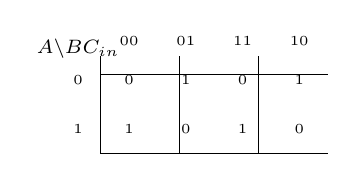
\begin{tikzpicture}[x=0.72cm,y=0.62cm,font=\tiny]
  \draw (0,0) grid (4,2);
  \node at (0.5,2.3) {$00$}; \node at (1.5,2.3) {$01$};
  \node at (2.5,2.3) {$11$}; \node at (3.5,2.3) {$10$};
  \node at (0.5,1.5) {$0$}; \node at (1.5,1.5) {$1$};
  \node at (2.5,1.5) {$0$}; \node at (3.5,1.5) {$1$};
  \node at (0.5,0.5) {$1$}; \node at (1.5,0.5) {$0$};
  \node at (2.5,0.5) {$1$}; \node at (3.5,0.5) {$0$};
  \node at (-0.4,1.5) {$0$}; \node at (-0.4,0.5) {$1$};
  \node at (-0.4,2.15) {\scriptsize $A{\backslash}BC_{in}$};
\end{tikzpicture}
\par\vspace{2pt}{\scriptsize Sum: no two 1-cells adjacent (parity).}
\end{minipage}
\hfill
\begin{minipage}{0.48\linewidth}
\centering
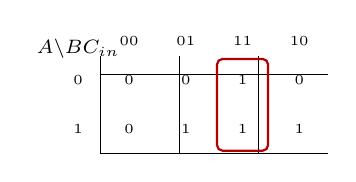
\begin{tikzpicture}[x=0.72cm,y=0.62cm,font=\tiny]
  \draw (0,0) grid (4,2);
  \node at (0.5,2.3) {$00$}; \node at (1.5,2.3) {$01$};
  \node at (2.5,2.3) {$11$}; \node at (3.5,2.3) {$10$};
  \node at (0.5,1.5) {$0$}; \node at (1.5,1.5) {$0$};
  \node at (2.5,1.5) {$1$}; \node at (3.5,1.5) {$0$};
  \node at (0.5,0.5) {$0$}; \node at (1.5,0.5) {$1$};
  \node at (2.5,0.5) {$1$}; \node at (3.5,0.5) {$1$};
  \node at (-0.4,1.5) {$0$}; \node at (-0.4,0.5) {$1$};
  \node at (-0.4,2.15) {\scriptsize $A{\backslash}BC_{in}$};
  \draw[thick,red!70!black,rounded corners=2pt] (2.05,0.06) rectangle (2.95,1.94);
\end{tikzpicture}
\par\vspace{2pt}{\scriptsize Carry: one real 2-cell group ($BC_{in}$).}
\end{minipage}
\caption{K-maps for the full adder.}
\label{fig:kmaps}
\end{figure}

$\mathrm{Sum}$'s on-set is one bipartition class of $Q_3$ (odd Hamming
weight), so no two of its cells are ever adjacent -- every group is a
single cell (Proposition~\ref{prop:parity}). $\mathrm{Carry}$'s one real
group, $BC_{in}$, is literally a cube edge; growing a group
(Section~\ref{sec:disjoint}) is walking from a vertex along edges into a
larger sub-cube for as long as every vertex reached stays in the on-set.

% =====================================================================
\section{Disjoint Cube Covers}
\label{sec:disjoint}
% =====================================================================

A classical K-map lets groups overlap: $A+B$ is normally read as two
overlapping groups, one for $A$ and one for $B$, with $AB=11$ covered by
both. That is sound for a circuit that \emph{sets} its output, but every
gate in Definition~\ref{def:gates} \emph{flips} its target -- a cell
covered by two groups is flipped twice and cancels to $0$. Table
\ref{tab:orbug} makes this concrete: naively wiring \code{cx(B,Out)} then
\code{cx(A,Out)} for $\mathrm{Out}=A+B$ gives the wrong answer on
$A{=}B{=}1$.

\begin{table}[t]
\centering
\caption{Naive overlapping-group OR is wrong on $A{=}B{=}1$.}
\label{tab:orbug}
\begin{tabular}{cc|cc|c}
\toprule
$A$&$B$& after \code{cx(B,\_)} & after \code{cx(A,\_)} & expected $A{+}B$\\
\midrule
0&0&0&0&0\\
0&1&1&1&1\\
1&0&0&1&1\\
1&1&1&\textcolor{red}{0}&\textcolor{red}{1}\\
\bottomrule
\end{tabular}
\end{table}

The correct, disjoint synthesis instead uses groups $B{=}1$ (any $A$) and
$A{=}1,B{=}0$: \code{cx(B,Out)}; $X(B)$; \code{ccx(A,B,Out)}; $X(B)$ --
since the two groups share no input pattern, at most one gate fires per
row.

\begin{algorithm}[t]
\caption{\Algo{GrowCube}$(seed,\mathit{remaining})$}
\label{alg:grow}
\begin{algorithmic}[1]
\State $p \gets seed$
\For{$i \gets 1$ \textbf{to} $n$}
  \If{$p_i={-}$} \textbf{continue} \EndIf
  \State $p' \gets p$ with position $i$ set to ${-}$
  \If{$\llbracket p' \rrbracket \subseteq \mathit{remaining}$} $p \gets p'$ \EndIf
\EndFor
\State \Return $p$
\end{algorithmic}
\end{algorithm}
\begin{algorithm}[t]
\caption{\Algo{DisjointCover}$(S)$}
\label{alg:cover}
\begin{algorithmic}[1]
\State $\mathit{remaining} \gets S$; $\mathit{selected} \gets \langle\rangle$
\While{$\mathit{remaining} \ne \emptyset$}
  \State $seed \gets \min(\mathit{remaining})$
  \State $p \gets \textsc{GrowCube}(seed,\mathit{remaining})$
  \State append $p$ to $\mathit{selected}$; $\mathit{remaining} \gets \mathit{remaining}\setminus\llbracket p\rrbracket$
\EndWhile
\State \Return $\mathit{selected}$
\end{algorithmic}
\end{algorithm}

\begin{theorem}[Exactness and disjointness]
\label{thm:exactness}
For $S\subseteq\{0,1\}^n$, let $p_1,\dots,p_r$ be \Algo{DisjointCover}$(S)$'s
output. Then $\llbracket p_i\rrbracket \cap \llbracket p_j\rrbracket=\emptyset$
for $i\ne j$, and $\bigcup_i \llbracket p_i\rrbracket = S$.
\end{theorem}
\begin{proof}
Let $R_k$ be \textit{remaining} before iteration $k$ ($R_1=S$). By
induction, $R_k=S\setminus\bigcup_{i<k}\llbracket p_i\rrbracket$ and
$\llbracket p_k\rrbracket\subseteq R_k$: \Algo{GrowCube} only accepts a
relaxation checked to keep the cube inside its argument, starting from
$seed\in R_k$. This gives disjointness inductively; line 6 maintains the
invariant. The loop halts when $R_{r+1}=\emptyset$, giving exactness.
Since $seed\in\llbracket p_k\rrbracket$ always, $|R_{k+1}|\le|R_k|-1$, so
termination is within $|S|$ iterations.
\end{proof}
Validated over $2000$ randomized on-sets ($n\le 6$), zero violations.

\section{From Terms to Circuits}
\label{sec:terms}

Each term becomes one multi-controlled $X$ gate (\code{\_emit\_term}):

\begin{center}
\small
\begin{tabular}{@{}ll@{}}
\toprule
Term & Gate(s)\\
\midrule
$1$ (no vars) & unconditional $X$\\
one var, e.g.\ $B$ & CNOT\\
$k{\ge}2$ vars, all uncomplemented & $k$-controlled Toffoli\\
$k{\ge}2$ vars, some complemented & $X$-sandwich around Toffoli\\
\bottomrule
\end{tabular}
\end{center}

\begin{theorem}[Correctness of synthesis]
\label{thm:correctness}
Let $f:\{0,1\}^n\to\{0,1\}^m$, and $C$ the circuit from applying
\Algo{DisjointCover} to each output and translating every term as above.
For every $x$, running $C$ on $(x,0^m)$ terminates in $(x,f(x))$.
\end{theorem}
\begin{proof}
For output $j$ with terms $p_1,\dots,p_{r_j}$, each term's gates flip wire
$n{+}j$ iff $x\in\llbracket p_i\rrbracket$ ($X$-sandwiches cancel
otherwise). By Theorem~\ref{thm:exactness}(i), the $\llbracket p_i
\rrbracket$ are disjoint, so wire $n{+}j$ flips once iff $x$ is in the
on-set (Theorem~\ref{thm:exactness}(ii)), giving $f_j(x)$ from $0$.
Different outputs write disjoint wires; no gate targets an input wire.
\end{proof}

Figure~\ref{fig:fulladder} shows the complete full-adder circuit built
directly from Theorem~\ref{thm:correctness}'s construction: $4$ disjoint
terms for $\mathrm{Sum}$ (a full parity split, so every term has all $3$
variables specified) and $3$ for $\mathrm{Carry}$. Counting each $X$,
CNOT, and Toffoli as one elementary gate per Definition~\ref{def:gates}
gives $16$ gates for $\mathrm{Sum}$ and $7$ for $\mathrm{Carry}$, $23$ in
total as emitted. The figure also shows the redundancy this paper's
peephole pass removes: for example, the first two $\mathrm{Sum}$ terms
leave two consecutive $X$ gates on wire $A$, which cancel. After
$X$-cancellation (Section~\ref{sec:xcancel}) the same circuit has $19$
gates.

\begin{figure*}[t]
\centering
\begin{quantikz}[column sep=4pt]
\lstick{$A$} & \gate{X} & \ctrl{1} & \gate{X} & \gate{X} & \ctrl{1} & \gate{X} & \qw & \ctrl{1} & \qw & \ctrl{1} & \qw & \qw & \ctrl{1} & \qw & \qw & \ctrl{1} & \qw & \qw \\
\lstick{$B$} & \gate{X} & \ctrl{1} & \gate{X} & \qw & \ctrl{1} & \qw & \gate{X} & \ctrl{1} & \gate{X} & \ctrl{1} & \ctrl{1} & \gate{X} & \ctrl{1} & \gate{X} & \qw & \ctrl{1} & \qw & \qw \\
\lstick{$C_{in}$} & \qw & \ctrl{1} & \qw & \gate{X} & \ctrl{1} & \gate{X} & \gate{X} & \ctrl{1} & \gate{X} & \ctrl{1} & \ctrl{2} & \qw & \ctrl{2} & \qw & \gate{X} & \ctrl{2} & \gate{X} & \qw \\
\lstick{$\mathrm{Sum}=\ket0$} & \qw & \targ{} & \qw & \qw & \targ{} & \qw & \qw & \targ{} & \qw & \targ{} & \qw & \qw & \qw & \qw & \qw & \qw & \qw & \qw \\
\lstick{$\mathrm{Carry}=\ket0$} & \qw & \qw & \qw & \qw & \qw & \qw & \qw & \qw & \qw & \qw & \targ{} & \qw & \targ{} & \qw & \qw & \targ{} & \qw & \qw
\end{quantikz}
\caption{The complete full-adder circuit as emitted: all gates for $\mathrm{Sum}$'s four terms, then all gates for $\mathrm{Carry}$'s three terms ($23$ elementary gates; $19$ after $X$-cancellation, Section~\ref{sec:xcancel}).}
\label{fig:fulladder}
\end{figure*}

\section{Verifying the Circuit}
\label{sec:verify}

Because every gate acts on a basis state exactly as classically, a
classical replay (\code{simulate}) is an \emph{exact} check:
\code{simulate}$(C,x)=f(x)$ for every $x$ follows directly from
Theorem~\ref{thm:correctness}. \code{verify\_circuit} runs this for every
truth-table row. On $2000$ random truth tables it accepted every
synthesized circuit and rejected every one of them when checked against
the same table with one output bit flipped.

% =====================================================================
\section{Relevance to Quantum Devices}
\label{sec:devices}
% =====================================================================

This section fixes a concrete decomposition from our circuits to the
operations a device executes, and uses it to state why gate count is the
right quantity to minimize.

\subsection{From elementary gates to native and fault-tolerant cost}
Every gate in Definition~\ref{def:gates} has a standard, fixed-size
decomposition. An unconditional $X$ and a CNOT are already native on
essentially every gate-model platform. A $k$-controlled Toffoli
decomposes, using Barenco et al.'s construction~\cite{barenco1995}, into
$O(k)$ CNOT and single-qubit gates with one borrowed ancilla, or, for a
small, fixed number of controls, into a known constant number of
two-qubit gates and single-qubit rotations; on a fault-tolerant target
built from Clifford+T, the standard $2$-control Toffoli costs exactly $7$
T gates and $6$ CNOTs~\cite{barenco1995,nielsen2000}, and larger
multi-controlled gates decompose recursively into that primitive. The
\emph{quantum cost} metric used throughout the reversible-logic
literature, and by RevLib~\cite{revlib2008} specifically, assigns an
NOT/CNOT a cost of $1$ and a $k$-controlled Toffoli a cost of
$2^{k+1}-3$ for $k\ge 1$, matching this decomposition's two-qubit gate
count up to a small constant. We report this metric alongside
elementary gate count throughout Section~\ref{sec:benchmarks}.

\subsection{Why this gate set, specifically}
Definition~\ref{def:gates} is the positive-control multiple-control
Toffoli (MCT) library, written \texttt{t1}, \texttt{t2}, \dots\ in
RevLib's \texttt{.real} format, so gate counts compare gate for gate with
published MCT circuits, NOT gates included. It is also the granularity at
which a backend transpiler counts: a control that fires on $\ket 0$ is
compiled to an $X$-sandwiched positive control, exactly what
Section~\ref{sec:terms} emits and Section~\ref{sec:xcancel} cleans up.
Our construction is \emph{out-of-place} ($n+m$ lines, inputs preserved),
whereas published circuits for reversible functions are usually
\emph{in-place} on $n$ lines (Section~\ref{sec:head-to-head}).

\subsection{Where this sits in Grover and Shor pipelines}
A Grover oracle applies the synthesized circuit and its inverse once per
amplitude-amplification iteration, typically $O(\sqrt{2^n})$ times, so a
per-call gate-count or T-count reduction compounds with the iteration
count. A Shor-style modular adder chains one full-adder circuit
(Section~\ref{sec:terms}) per bit of the modulus, so the per-adder
quantum cost of Section~\ref{sec:benchmarks} multiplies into the depth of
the arithmetic block, which must fit within the device's $T_2$. In both
cases the quantity minimized here, gate count and through the
decomposition above quantum cost, bounds whether the circuit is
executable on current hardware.

% =====================================================================
\section{Output-Level Optimizations}
\label{sec:optim}
% =====================================================================

\subsection{Sharing a term between outputs}
When two or more outputs need the exact same term with $2{+}$ controls,
\code{synthesize} computes it once into a scratch ancilla, CNOTs it into
each output that needs it, then uncomputes the ancilla by re-running the
same gate.

\begin{lemma}[Sharing]
\label{lem:sharing}
Let $p$ be shared by output set $J$, computed into ancilla $a$ ($0$
initially), copied to each $j\in J$ by a CNOT on $a$, then uncomputed by
re-applying the compute step. For any $x$: (i) $a$ returns to $0$; (ii)
each $j\in J$ is flipped iff $x\in\llbracket p\rrbracket$.
\end{lemma}
\begin{proof}
The compute step sets $a\gets[x\in\llbracket p\rrbracket]$ (Theorem
\ref{thm:correctness}'s single-term case). Copy steps flip $j$
conditioned on $a$ without touching $a$ or input wires. The uncompute
step recomputes the same indicator and XORs it into $a$ again, giving
$a\gets 0$.
\end{proof}
This never triggers for the full adder's own $\mathrm{Sum}$/$\mathrm{Carry}$
(no shared terms), which is why Figure~\ref{fig:fulladder} uses no
ancilla. It rarely pays off: for two outputs it costs $2c+2$ gates
against $2c$ for a $c$-gate term. On the $2000$ random truth tables of
Section~\ref{sec:xcancel} the gate-count rule never selects it and the
cancellation-aware rule does in $0.4\%$; no benchmark circuit uses an
ancilla.

\subsection{Deriving one output from another}
An earlier output's wire keeps its value, so a later output can be built
by CNOTing that wire in and XORing in the difference. The difference
$r(x)=f_j(x)\oplus f_k(x)$ gets its own disjoint cover and cost; this
replaces building $f_k$ directly only when strictly cheaper.

\begin{lemma}[Derivation]
\label{lem:derive}
Suppose wire $j$ holds $f_j(x)$. Build (initially-$0$) wire $k$ by (i) a
CNOT from $j$ to $k$, then (ii) \Algo{DisjointCover}$(r)$'s gates targeting
$k$. Then wire $k$ ends at $f_k(x)$, and no other wire is modified.
\end{lemma}
\begin{proof}
After (i), $k$ holds $f_j(x)$. Step (ii), by Theorem
\ref{thm:correctness}'s single-output case applied to $r$, flips $k$ iff
$r(x)=1$, using only input wires as controls. Final value:
$f_j(x)\oplus r(x) = f_k(x)$.
\end{proof}

\code{synthesize} processes outputs by increasing direct cost, so a later
output can borrow from any cheaper earlier one. Of the $2000$ random truth
tables of Section~\ref{sec:xcancel}, $1326$ have two or more outputs;
choosing by gate count, derivation is used in $48.7\%$ of these and then
cuts gate count before cancellation by $22.5\%$ on average, and every
circuit passes exhaustive replay.

\textbf{Ripple-carry example.} Chaining two full-adder bits with all four
internal signals exposed --
$S_0=A_0{\oplus}B_0{\oplus}C_{in}$, $C_0=A_0B_0{+}B_0C_{in}{+}A_0C_{in}$,
$S_1=A_1{\oplus}B_1{\oplus}C_0$, $\mathrm{Cout}=A_1B_1{+}B_1C_0{+}A_1C_0$
-- in one \code{synthesize} call lets derivation find that
$S_1\oplus C_0=A_1\oplus B_1$, the standard full-adder identity
``sum = inputs XOR incoming carry.'' Table~\ref{tab:adder2} shows the result,
checked against all $32$ rows: derivation very nearly halves total gate
count, from $126$ elementary gates to $64$. $X$-cancellation
(Section~\ref{sec:xcancel}) alone takes the direct circuit from $126$ to
$86$ gates, and derivation chosen by gate count followed by cancellation
reaches $58$. Choosing by gate count \emph{after} cancellation
(Section~\ref{sec:xcancel}) builds $S_0$ directly and derives
$\mathrm{Cout}$ from $C_0$ instead: $65$ gates before cancellation but
$47$ after, a $63\%$ reduction from the direct circuit. Term ordering
(Section~\ref{sec:order}) then reaches $31$.

\begin{table}[t]
\centering
\caption{Two-bit ripple-carry adder: elementary gate cost per output before $X$-cancellation, with derivation chosen by gate count before or after cancellation (base output in parentheses).}
\label{tab:adder2}
\begin{tabular}{@{}lrrr@{}}
\toprule
Output & Direct & Before-$X$ rule & After-$X$ rule\\
\midrule
$S_0$ & 16 & 15 ($C_0$) & 16\\
$C_0$ & 7 & 7 & 7\\
$S_1$ & 68 & 7 ($C_0$) & 7 ($C_0$)\\
$\mathrm{Cout}$ & 35 & 35 & 35 ($C_0$)\\
\midrule
Total & 126 & 64 & 65\\
After $X$-cancellation & 86 & 58 & 47\\
\bottomrule
\end{tabular}
\end{table}

\subsection{Cancelling adjacent \texorpdfstring{$X$}{X} gates}
\label{sec:xcancel}
Every term with a complemented literal is wrapped in $X$ gates on those
wires (Section~\ref{sec:terms}), so consecutive terms often leave an $X$
on wire $w$ followed, with only gates that do not use $w$ as a control in
between, by another $X$ on $w$. Since $X^2=I$ the pair is redundant. The
\emph{$X$-cancellation pass} scans the gate list, and for each $X_w$ looks
forward for the next $X_w$; if every gate in between commutes with $X_w$
it deletes both, repeating until no pair remains. It never increases gate
count.

\begin{lemma}[$X$-cancellation]
\label{lem:xcancel}
Let a circuit contain $X_w, h_1,\dots,h_r, X_w$ in sequence, where each
$h_i$ either does not involve wire $w$ or has $w$ as its \emph{target}
(never as a control). Deleting both $X_w$ gates leaves the circuit's action
unchanged.
\end{lemma}
\begin{proof}
$X_w$ commutes with every gate acting on other wires. It also commutes
with a gate $C^kX_{c_1,\dots,c_k\to w}$: both flip $w$, and the condition
on $c_1,\dots,c_k$ is unaffected by flipping $w$. Moving the first $X_w$
rightward past $h_1,\dots,h_r$ makes it adjacent to the second, and
$X_wX_w=I$.
\end{proof}

On the full adder the pass reduces $23$ gates to $19$. Over $2000$ random
truth tables ($2\le n\le 4$, $1\le m\le 3$) it changed the gate count of
$47\%$ of the disjoint-cover circuits, by $9.7\%$ on average, all
re-verified by exhaustive replay.
Its effect is larger on structured functions (Table~\ref{tab:counts}):
for the $4$-bit equality comparator every term is a fully specified
minterm, so almost every $X$-sandwich boundary cancels and the pass
removes $47\%$ of the gates, whereas sharing and derivation find nothing
to exploit there. The order in which terms are emitted also matters;
Section~\ref{sec:order} exploits it.

\textbf{Interaction with derivation and sharing.} Chosen by gate count
\emph{before} cancellation, derivation and sharing do not always combine
well with the pass: on the full adder, derivation $+$ cancellation gives
$22$ gates, worse than cancellation alone ($19$), and across the random
trials above that pipeline was worse than cover $+$ cancellation in
$2.4\%$ of cases. We therefore choose both by gate count \emph{after}
cancellation: each candidate for an output (built directly, or derived
from an earlier output) is scored by the cancelled length of the circuit
built so far followed by it, and a shared term is kept only if it
shortens the cancelled circuit. $X$ gates sit only on input wires, so by
Lemma~\ref{lem:xcancel} the cancelled length is the number of
multi-controlled gates plus, for each wire, the parity of the $X$ gates
between consecutive control uses -- one pass, no rewriting. The pipeline
returns the plain cover circuit, or the before-cancellation rule's
circuit, when either is smaller after cancellation, so it is never worse
than either; without this fallback it is worse than cover $+$
cancellation in $0.3\%$ of the random trials, and on the benchmarks the
fallback is never used. The full adder now keeps $19$ gates, the ripple
adder reaches $47$ rather than $58$, the multiplier $97$ rather than $98$,
and the rest are unchanged. Gate count, not quantum cost, is minimized:
the full adder's $Q$-cost rises from $82$ to $95$.

\subsection{Ordering terms}
\label{sec:order}
Call each term's gate sequence, each derivation CNOT, and each shared
term's compute/copy/uncompute sequence a \emph{block}. Each block XORs a
function of the wires it reads into wires it does not read: a term block
reads inputs, a derivation CNOT reads its base output, and a shared block
(its ancilla restored by Lemma~\ref{lem:sharing}) reads inputs.

\begin{lemma}[Reordering]
\label{lem:reorder}
Any order of a circuit's blocks in which each derivation CNOT from output
$i$ follows every block that writes wire $n{+}i$ computes the same
function as the emitted order.
\end{lemma}
\begin{proof}
Two blocks commute when neither writes a wire the other reads: both
orders XOR the same values into the written wires. The only blocks that
read a non-input wire are derivation CNOTs, so the only non-commuting
pairs are a CNOT from output $i$ and a block writing $n{+}i$, and the
emitted order already places every such writer first. Any order
satisfying the stated constraint is reached from the emitted one by
swapping adjacent commuting blocks.
\end{proof}

The heuristic appends, greedily, the admissible block giving the
shortest cancelled prefix, then moves single blocks to other positions
while the move satisfies Lemma~\ref{lem:reorder} and shortens the
cancelled circuit. It starts from the emitted and the greedy order and is
applied to the cancellation-aware, plain cover, and
before-cancellation-rule circuits; the shortest result is kept and
re-verified by exhaustive replay. As a reference, the cancelled length
accumulates block by block given the set of placed blocks and each input
wire's current $X$ parity, so dynamic programming over these states gives
the exact optimum in $O(2^B 2^n B)$ time for $B$ blocks (used here up to
$B=16$). On the full adder's seven cover terms it agrees with exhaustive
search over all $7!=5040$ orders: $15$ gates, reached by $144$ of them.

\begin{table}[t]
\centering
\caption{Gates after $X$-cancellation without and with term ordering;
Opt.\ is the exact best order of the same candidate circuits (-- where
$B>16$). Right: gates\,/\,$Q$-cost of our final circuit (full$+X+$ord.)
and of tweedledum~1.1.1 on the same $n+m$ lines (Section~\ref{sec:tools}).}
\label{tab:order}
\footnotesize
\setlength{\tabcolsep}{2.6pt}
\begin{tabular}{@{}lrrrrrrrr@{}}
\toprule
& \multicolumn{5}{c}{Term ordering} & \multicolumn{3}{c}{Gates / $Q$-cost}\\
\cmidrule(lr){2-6}\cmidrule(l){7-9}
Function & C$+X$ & $+$ord. & F$+X$ & $+$ord. & Opt. & Ours & PKRM & PPRM\\
\midrule
AND & 1 & 1 & 1 & 1 & 1 & 1/5 & 1/5 & 1/5\\
OR & 4 & 4 & 4 & 4 & 4 & 4/8 & 4/8 & 3/7\\
XOR & 6 & 6 & 6 & 6 & 6 & 6/14 & 2/2 & 2/2\\
NAND & 6 & 6 & 6 & 6 & 6 & 6/10 & 6/10 & 2/6\\
Half adder & 7 & 7 & 6 & 6 & 6 & 6/14 & 3/7 & 3/7\\
Full adder & 19 & 15 & 19 & 14 & 14 & 14/74 & 10/22 & 6/18\\
2-bit ripple & 86 & 54 & 47 & 31 & -- & 31/411 & 34/142 & 18/118\\
BCD$\to$XS-3 & 36 & 24 & 28 & 22 & 22 & 22/190 & 45/257 & 32/292\\
$3{\times}3$ mult. & 123 & 69 & 97 & 60 & -- & 60/1920 & 80/936 & 27/919\\
4-bit compar. & 76 & 52 & 76 & 52 & 48 & 52/8180 & 24/472 & 81/1009\\
\texttt{3\_17} & 22 & 16 & 15 & 13 & 13 & 13/37 & 15/31 & 14/30\\
\bottomrule
\end{tabular}
\end{table}

Ordering never increases the count (Table~\ref{tab:order}); it takes
the full adder to $14$ by reordering the derivation-based circuit. It is
not always optimal: the comparator stops at $52$ against an exact $48$. On the $2000$ random truth tables it removes a further $9.4\%$
of the gates on average and reaches the exact optimum in $1806$ of the
$1904$ circuits ($94.9\%$) where that optimum was computed.

% =====================================================================
\section{Complexity}
\label{sec:complexity}
% =====================================================================

Without minimization, gate count is the number of $1$-rows across all
outputs, $O(2^n m)$ worst case. With disjoint-cover minimization, term
count per output is at most its on-set size and can be as low as $1$.

\begin{proposition}[Parity worst case]
\label{prop:parity}
For the $n$-bit parity function ($n{\ge}1$), \Algo{DisjointCover} returns
exactly $2^{n-1}$ singleton terms.
\end{proposition}
\begin{proof}
Flipping one coordinate flips parity, so any two on-set elements differ in
$\ge 2$ coordinates -- no cube of dimension $\ge 1$ fits inside the
on-set. The balanced on-set has $2^{n-1}$ elements.
\end{proof}
Realized exactly by $\mathrm{Sum}$: $2^{3-1}{=}4$ terms. Table
\ref{tab:counts} gives gate counts for all eleven functions of this paper
(the six built-in presets and those of Section~\ref{sec:benchmarks}): \emph{Raw}
is one term per on-set row, \emph{Cover} is \Algo{DisjointCover}, and the
$+X$ columns apply the $X$-cancellation pass of
Section~\ref{sec:xcancel}. All counts are elementary gates ($X$, CNOT,
Toffoli) from the actual emitted circuit, each verified by exhaustive
classical replay.

\begin{table}[t]
\centering
\caption{Elementary gate count before and after ($+X$) $X$-cancellation.
Full $=$ derivation $+$ sharing chosen after cancellation.}
\label{tab:counts}
\footnotesize
\setlength{\tabcolsep}{3.5pt}
\begin{tabular}{@{}lrrrrrrrr@{}}
\toprule
Function & $n$ & $m$ & Raw & Raw$+X$ & Cover & Cover$+X$ & Full & Full$+X$\\
\midrule
AND & 2 & 1 & 1 & 1 & 1 & 1 & 1 & 1\\
OR & 2 & 1 & 7 & 7 & 4 & 4 & 4 & 4\\
XOR & 2 & 1 & 6 & 6 & 6 & 6 & 6 & 6\\
NAND & 2 & 1 & 11 & 9 & 6 & 6 & 6 & 6\\
Half adder & 2 & 2 & 7 & 7 & 7 & 7 & 6 & 6\\
Full adder & 3 & 2 & 26 & 22 & 23 & 19 & 23 & 19\\
2-bit ripple & 5 & 4 & 332 & 202 & 126 & 86 & 65 & 47\\
BCD$\to$XS-3 & 4 & 4 & 122 & 64 & 66 & 36 & 50 & 28\\
$3{\times}3$ mult. & 6 & 6 & 615 & 343 & 159 & 123 & 123 & 97\\
4-bit compar. & 8 & 1 & 144 & 76 & 144 & 76 & 144 & 76\\
\texttt{3\_17} & 3 & 3 & 48 & 32 & 28 & 22 & 17 & 15\\
\bottomrule
\end{tabular}
\end{table}

% =====================================================================
\section{Benchmark Evaluation}
\label{sec:benchmarks}
% =====================================================================

All numbers come from a Python implementation of
Algorithms~\ref{alg:grow}--\ref{alg:cover}, Lemmas~\ref{lem:sharing}--%
\ref{lem:reorder}, and the gate set of Definition~\ref{def:gates}; every
circuit, before and after cancellation, was checked against its truth
table on all $2^n$ input rows, and all ancillas were checked to return to
$\ket 0$.

\subsection{Broader functions}
Besides the presets, the ripple adder, and \texttt{3\_17}, we use
\textbf{BCD-to-Excess-3} (4 inputs, 4 outputs), a standard small
benchmark; a \textbf{$3\times 3$-bit multiplier} (6 inputs, 6 outputs),
an arithmetic block of the kind Shor-style modular multiplication chains;
and a \textbf{4-bit equality comparator} (8 inputs, 1 output), a wide
single-output predicate of the shape a Grover oracle needs.

Disjoint-cover minimization alone cuts gate count substantially ($74\%$
on the multiplier), and $X$-cancellation compounds on top of it ($159\to
123$ on the multiplier, $66\to 36$ on BCD-to-Excess-3). Derivation and
sharing help where outputs share structure -- several of the multiplier's
product bits are cheaper to derive from another product bit than to build
from scratch -- bringing the multiplier from $615$ raw gates to $97$, and
term ordering to $60$ (Table~\ref{tab:order}). The comparator is the
instructive case: its on-set has no adjacent cells, so the cover,
sharing, and derivation return the unminimized count, and the entire gain
($144\to76$, $47\%$) comes from $X$-cancellation, which term ordering
extends to $52$ ($64\%$).

\subsection{Head-to-head against published circuits}
\label{sec:head-to-head}
We compare against published circuits for two RevLib
benchmarks~\cite{revlib2008}, quoted from RevLib rather than re-run, and
against tweedledum (Section~\ref{sec:tools}). \texttt{3\_17}
is a $3$-input, $3$-output \emph{bijection}, listed on RevLib as a known
worst case for Miller--Maslov--Dueck transformation-based synthesis
\cite{miller2003}; the published MMD circuit has $6$ gates on $3$ lines.
\texttt{rd32} is the $1$-bit adder, i.e.\ our full adder; the best MCT
circuit listed on RevLib has $4$ gates on $4$ lines (three inputs plus one
constant-$0$ line), with garbage outputs permitted. We took each
function's specification from RevLib. All entries use the
positive-control MCT library of Definition~\ref{def:gates}, so gate counts
and quantum costs are directly comparable, except the GWDD entry, which
uses the elementary quantum-gate library ($V$, $V^\dagger$, CNOT) and is
comparable only through quantum cost.

\begin{table}[t]
\centering
\caption{Head-to-head against published circuits and tweedledum; this
work is full$+X+$ord.\ (Table~\ref{tab:order}). $Q$-cost uses the
$2^{k+1}-3$ rule of Section~\ref{sec:devices} (NOT, CNOT $=1$).}
\label{tab:head2head}
\small
\begin{tabular}{@{}llrrr@{}}
\toprule
Function & Method & Lines & Gates & $Q$-cost\\
\midrule
\texttt{3\_17} & MMD, MCT \cite{miller2003} & 3 & 6 & 14\\
 & GWDD exact, EQ lib.\ \cite{grosse2008} & 3 & 10 & 10\\
 & tweedledum transformation & 3 & 7 & 15\\
 & tweedledum PPRM & 6 & 14 & 30\\
 & This work & 6 & 13 & 37\\
\midrule
\texttt{rd32} & Best MCT on RevLib \cite{revlib2008} & 4 & 4 & 12\\
 & tweedledum PPRM & 5 & 6 & 18\\
 & This work & 5 & 14 & 74\\
\bottomrule
\end{tabular}
\end{table}

Table~\ref{tab:head2head} shows that our construction is substantially
larger than the published circuits: on \texttt{3\_17}, $13$ gates and
$Q$-cost $37$ against $6$ and $14$ ($2.2\times$ and $2.6\times$); on
\texttt{rd32}, $14$ gates and $Q$-cost $74$ against $4$ and $12$
($3.5\times$ and $6.2\times$). On our line count, tweedledum's PPRM
circuit has one gate more than ours on \texttt{3\_17} but lower $Q$-cost,
and is far smaller on \texttt{rd32}; its transformation-based synthesis
gives $7$ gates in place on \texttt{3\_17}, close to the published MMD
circuit. Three causes are visible. First, our circuits
are out-of-place: for a bijection like \texttt{3\_17}, in-place synthesis
on $3$ lines is possible and uses half the lines, and for \texttt{rd32}
the published circuit exploits garbage outputs and overwrites its inputs,
which ours preserves. Second, search-based methods find shared structure
that a cube cover, which treats each output separately before derivation,
does not. Third, our passes are greedy. We do not claim
competitiveness on gate count or quantum cost; the construction offers a
correctness argument short enough to check by hand
(Theorems~\ref{thm:exactness}--\ref{thm:correctness},
Lemmas~\ref{lem:sharing}--\ref{lem:reorder}) and preserved inputs.

\subsection{tweedledum on all functions}
\label{sec:tools}
We ran tweedledum~1.1.1~\cite{schmitt2022}: its PKRM and PPRM synthesizers, which build each
output as an exclusive-or sum of products on its own line ($n+m$ lines,
as ours), on all eleven functions, and its transformation-based
synthesizer in place on the bijection \texttt{3\_17}. We rewrite each
negative control as an $X$-sandwich, apply our cancellation pass, verify
every circuit by exhaustive replay, and count gates in the library of
Definition~\ref{def:gates}.

tweedledum's better circuit has fewer gates than ours on eight of the
eleven functions (Table~\ref{tab:order}); AND ties, and ours has
fewer gates on BCD-to-Excess-3 ($22$ against $32$) and \texttt{3\_17}
($13$ against $14$). Ours has lower $Q$-cost only on BCD-to-Excess-3
($190$ against $257$). The largest gap is the comparator's $Q$-cost,
$8180$ against $472$: every term of our cover is an $8$-control minterm,
while an exclusive-or form shares structure across terms. Counted in
tweedledum's native mixed-polarity library, where a negative control is
free, its circuits are smaller still (PKRM uses $15$ gates on
BCD-to-Excess-3).

% =====================================================================
\section{Limitations}
\label{sec:limitations}
% =====================================================================

\Algo{DisjointCover} is greedy, not globally optimal, and can occasionally
choose more total literals than an exhaustive search would. Term sharing
fires only on exact pattern matches and almost never pays off; derivation
considers one base output at a time, in increasing-cost order. Both are
chosen greedily after $X$-cancellation but before term ordering, and for
gate count rather than quantum cost. Term ordering is a local search: it
misses the exact optimum on the comparator and in $5.1\%$ of random
trials, and the exact optimum is out of reach for the ripple adder and
the multiplier.
Neither optimization decomposes
$k$-controlled Toffolis into elementary gates beyond the cost formula of
Section~\ref{sec:devices}; actual transpilation is left to the target
backend. As a restricted case of ESOP, a disjoint cube cover gives up
the smaller circuits a general ESOP search can find.
Sections~\ref{sec:head-to-head}--\ref{sec:tools} quantify the resulting
gap. Closing it
-- cost-aware cube growth, non-disjoint exclusive-or terms, and an
in-place variant for reversible functions -- is future work. Finally, the
RevLib circuits are quoted from their publications rather than
re-synthesized, we ran tweedledum but not RevKit, and our evaluation is
limited to functions with $n\le 8$.

% =====================================================================
\section{Conclusion}
% =====================================================================

Karnaugh-map grouping is built for a gate model that sets its output and
breaks, concretely, when applied to one that flips it instead. Requiring
groups to be disjoint fixes this with a short, elementary proof
(Theorem~\ref{thm:exactness}), and that one fix is sufficient, on its own,
to guarantee correct synthesis (Theorem~\ref{thm:correctness}). Sharing,
derivation, $X$-cancellation, and term ordering build on it without
weakening the guarantee (Lemmas~\ref{lem:sharing}--\ref{lem:reorder}),
taking a two-bit ripple-carry adder from $126$ to $31$ gates and a wide
comparator, where cover and derivation find nothing, from $144$ to $52$.

Gate count is tied to device cost through the standard Toffoli
decomposition (Section~\ref{sec:devices}), and on that measure the method
is not competitive with mature synthesizers: published in-place MCT
circuits are $2.2\times$ and $3.5\times$ smaller on \texttt{3\_17} and
\texttt{rd32}, and tweedledum's ESOP circuits have fewer gates on eight of
eleven functions. Its value is
instead as a minimal building block whose correctness argument is short
enough to verify by hand and is checked by exhaustive simulation, with clear
directions for closing the gap.

\begin{thebibliography}{99}
\bibitem{karnaugh1953} M. Karnaugh, ``The map method for synthesis of combinational logic circuits,'' \emph{Trans. AIEE, Part I}, vol.~72, no.~5, pp.~593--599, 1953.
\bibitem{quine1952} W. V. Quine, ``The problem of simplifying truth functions,'' \emph{Amer. Math. Monthly}, vol.~59, no.~8, pp.~521--531, 1952.
\bibitem{mccluskey1956} E. J. McCluskey, ``Minimization of Boolean functions,'' \emph{Bell Syst. Tech. J.}, vol.~35, no.~6, pp.~1417--1444, 1956.
\bibitem{toffoli1980} T. Toffoli, ``Reversible computing,'' in \emph{ICALP 1980}, LNCS vol.~85, Springer, pp.~632--644, 1980.
\bibitem{barenco1995} A. Barenco \emph{et al.}, ``Elementary gates for quantum computation,'' \emph{Phys. Rev. A}, vol.~52, no.~5, pp.~3457--3467, 1995.
\bibitem{nielsen2000} M. A. Nielsen and I. L. Chuang, \emph{Quantum Computation and Quantum Information}. Cambridge Univ. Press, 2000.
\bibitem{saeedi2013} M. Saeedi and I. L. Markov, ``Synthesis and optimization of reversible circuits---a survey,'' \emph{ACM Comput. Surv.}, vol.~45, no.~2, art.~21, 2013.
\bibitem{miller2003} D. M. Miller, D. Maslov, and G. W. Dueck, ``A transformation based algorithm for reversible logic synthesis,'' in \emph{Proc. 40th DAC}, pp.~318--323, 2003.
\bibitem{mishchenko2001} A. Mishchenko and M. Perkowski, ``Fast heuristic minimization of exclusive-sums-of-products,'' in \emph{Proc. 5th Int'l Reed-Muller Workshop (RM)}, pp.~242--250, 2001.
\bibitem{wille2009bdd} R. Wille and R. Drechsler, ``BDD-based synthesis of reversible logic for large functions,'' in \emph{Proc. 46th DAC}, pp.~270--275, 2009.
\bibitem{grosse2008} D. Gro{\ss}e, R. Wille, G. W. Dueck, and R. Drechsler, ``Exact synthesis of elementary quantum gate circuits for reversible functions with don't cares,'' in \emph{Proc. 38th Int'l Symp. on Multiple-Valued Logic (ISMVL)}, pp.~214--219, 2008.
\bibitem{sivarajah2020} S. Sivarajah, S. Dilkes, A. Cowtan, W. Simmons, A. Edgington, and R. Duncan, ``t$|$ket$\rangle$: A retargetable compiler for NISQ devices,'' \emph{Quantum Sci. Technol.}, vol.~6, no.~1, art.~014003, 2021.
\bibitem{qiskit2024} A. Javadi-Abhari \emph{et al.}, ``Quantum computing with Qiskit,'' arXiv:2405.08810, 2024.
\bibitem{amy2013} M. Amy, D. Maslov, M. Mosca, and M. Roetteler, ``A meet-in-the-middle algorithm for fast synthesis of depth-optimal quantum circuits,'' \emph{IEEE Trans. Comput.-Aided Design Integr. Circuits Syst.}, vol.~32, no.~6, pp.~818--830, 2013.
\bibitem{revlib2008} R. Wille, D. Gro{\ss}e, L. Teuber, G. W. Dueck, and R. Drechsler, ``RevLib: An online resource for reversible functions and reversible circuits,'' in \emph{Proc. 38th Int'l Symp. on Multiple-Valued Logic (ISMVL)}, pp.~220--225, 2008.
\bibitem{soeken2012revkit} M. Soeken, S. Frehse, R. Wille, and R. Drechsler, ``RevKit: An open source toolkit for the design of reversible circuits,'' in \emph{Reversible Computation 2011}, LNCS vol.~7165, Springer, pp.~64--76, 2012.
\bibitem{schmitt2022} B. Schmitt and G. De Micheli, ``tweedledum: A compiler companion for quantum computing,'' in \emph{Proc. DATE}, pp.~7--12, 2022.
\bibitem{wille2016syrec} R. Wille, E. Sch\"onborn, M. Soeken, and R. Drechsler, ``SyReC: A hardware description language for the specification and synthesis of reversible circuits,'' \emph{Integration}, vol.~53, pp.~39--53, 2016.

\end{thebibliography}

\end{document}
